\documentclass[]{article}
\usepackage{lmodern}
\usepackage{amssymb,amsmath}
\usepackage{ifxetex,ifluatex}
\usepackage{fixltx2e} % provides \textsubscript
\ifnum 0\ifxetex 1\fi\ifluatex 1\fi=0 % if pdftex
  \usepackage[T1]{fontenc}
  \usepackage[utf8]{inputenc}
\else % if luatex or xelatex
  \ifxetex
    \usepackage{mathspec}
  \else
    \usepackage{fontspec}
  \fi
  \defaultfontfeatures{Ligatures=TeX,Scale=MatchLowercase}
\fi
% use upquote if available, for straight quotes in verbatim environments
\IfFileExists{upquote.sty}{\usepackage{upquote}}{}
% use microtype if available
\IfFileExists{microtype.sty}{%
\usepackage{microtype}
\UseMicrotypeSet[protrusion]{basicmath} % disable protrusion for tt fonts
}{}
\usepackage[margin=1in]{geometry}
\usepackage{hyperref}
\hypersetup{unicode=true,
            pdftitle={Call Center Data},
            pdfauthor={Syed Rahman},
            pdfborder={0 0 0},
            breaklinks=true}
\urlstyle{same}  % don't use monospace font for urls
\usepackage{color}
\usepackage{fancyvrb}
\newcommand{\VerbBar}{|}
\newcommand{\VERB}{\Verb[commandchars=\\\{\}]}
\DefineVerbatimEnvironment{Highlighting}{Verbatim}{commandchars=\\\{\}}
% Add ',fontsize=\small' for more characters per line
\usepackage{framed}
\definecolor{shadecolor}{RGB}{248,248,248}
\newenvironment{Shaded}{\begin{snugshade}}{\end{snugshade}}
\newcommand{\KeywordTok}[1]{\textcolor[rgb]{0.13,0.29,0.53}{\textbf{#1}}}
\newcommand{\DataTypeTok}[1]{\textcolor[rgb]{0.13,0.29,0.53}{#1}}
\newcommand{\DecValTok}[1]{\textcolor[rgb]{0.00,0.00,0.81}{#1}}
\newcommand{\BaseNTok}[1]{\textcolor[rgb]{0.00,0.00,0.81}{#1}}
\newcommand{\FloatTok}[1]{\textcolor[rgb]{0.00,0.00,0.81}{#1}}
\newcommand{\ConstantTok}[1]{\textcolor[rgb]{0.00,0.00,0.00}{#1}}
\newcommand{\CharTok}[1]{\textcolor[rgb]{0.31,0.60,0.02}{#1}}
\newcommand{\SpecialCharTok}[1]{\textcolor[rgb]{0.00,0.00,0.00}{#1}}
\newcommand{\StringTok}[1]{\textcolor[rgb]{0.31,0.60,0.02}{#1}}
\newcommand{\VerbatimStringTok}[1]{\textcolor[rgb]{0.31,0.60,0.02}{#1}}
\newcommand{\SpecialStringTok}[1]{\textcolor[rgb]{0.31,0.60,0.02}{#1}}
\newcommand{\ImportTok}[1]{#1}
\newcommand{\CommentTok}[1]{\textcolor[rgb]{0.56,0.35,0.01}{\textit{#1}}}
\newcommand{\DocumentationTok}[1]{\textcolor[rgb]{0.56,0.35,0.01}{\textbf{\textit{#1}}}}
\newcommand{\AnnotationTok}[1]{\textcolor[rgb]{0.56,0.35,0.01}{\textbf{\textit{#1}}}}
\newcommand{\CommentVarTok}[1]{\textcolor[rgb]{0.56,0.35,0.01}{\textbf{\textit{#1}}}}
\newcommand{\OtherTok}[1]{\textcolor[rgb]{0.56,0.35,0.01}{#1}}
\newcommand{\FunctionTok}[1]{\textcolor[rgb]{0.00,0.00,0.00}{#1}}
\newcommand{\VariableTok}[1]{\textcolor[rgb]{0.00,0.00,0.00}{#1}}
\newcommand{\ControlFlowTok}[1]{\textcolor[rgb]{0.13,0.29,0.53}{\textbf{#1}}}
\newcommand{\OperatorTok}[1]{\textcolor[rgb]{0.81,0.36,0.00}{\textbf{#1}}}
\newcommand{\BuiltInTok}[1]{#1}
\newcommand{\ExtensionTok}[1]{#1}
\newcommand{\PreprocessorTok}[1]{\textcolor[rgb]{0.56,0.35,0.01}{\textit{#1}}}
\newcommand{\AttributeTok}[1]{\textcolor[rgb]{0.77,0.63,0.00}{#1}}
\newcommand{\RegionMarkerTok}[1]{#1}
\newcommand{\InformationTok}[1]{\textcolor[rgb]{0.56,0.35,0.01}{\textbf{\textit{#1}}}}
\newcommand{\WarningTok}[1]{\textcolor[rgb]{0.56,0.35,0.01}{\textbf{\textit{#1}}}}
\newcommand{\AlertTok}[1]{\textcolor[rgb]{0.94,0.16,0.16}{#1}}
\newcommand{\ErrorTok}[1]{\textcolor[rgb]{0.64,0.00,0.00}{\textbf{#1}}}
\newcommand{\NormalTok}[1]{#1}
\usepackage{graphicx,grffile}
\makeatletter
\def\maxwidth{\ifdim\Gin@nat@width>\linewidth\linewidth\else\Gin@nat@width\fi}
\def\maxheight{\ifdim\Gin@nat@height>\textheight\textheight\else\Gin@nat@height\fi}
\makeatother
% Scale images if necessary, so that they will not overflow the page
% margins by default, and it is still possible to overwrite the defaults
% using explicit options in \includegraphics[width, height, ...]{}
\setkeys{Gin}{width=\maxwidth,height=\maxheight,keepaspectratio}
\IfFileExists{parskip.sty}{%
\usepackage{parskip}
}{% else
\setlength{\parindent}{0pt}
\setlength{\parskip}{6pt plus 2pt minus 1pt}
}
\setlength{\emergencystretch}{3em}  % prevent overfull lines
\providecommand{\tightlist}{%
  \setlength{\itemsep}{0pt}\setlength{\parskip}{0pt}}
\setcounter{secnumdepth}{0}
% Redefines (sub)paragraphs to behave more like sections
\ifx\paragraph\undefined\else
\let\oldparagraph\paragraph
\renewcommand{\paragraph}[1]{\oldparagraph{#1}\mbox{}}
\fi
\ifx\subparagraph\undefined\else
\let\oldsubparagraph\subparagraph
\renewcommand{\subparagraph}[1]{\oldsubparagraph{#1}\mbox{}}
\fi

%%% Use protect on footnotes to avoid problems with footnotes in titles
\let\rmarkdownfootnote\footnote%
\def\footnote{\protect\rmarkdownfootnote}

%%% Change title format to be more compact
\usepackage{titling}

% Create subtitle command for use in maketitle
\newcommand{\subtitle}[1]{
  \posttitle{
    \begin{center}\large#1\end{center}
    }
}

\setlength{\droptitle}{-2em}

  \title{Call Center Data}
    \pretitle{\vspace{\droptitle}\centering\huge}
  \posttitle{\par}
    \author{Syed Rahman}
    \preauthor{\centering\large\emph}
  \postauthor{\par}
      \predate{\centering\large\emph}
  \postdate{\par}
    \date{04/24/2019}


\begin{document}
\maketitle

\subsection{Introduction}\label{introduction}

For this study, the data was obtained from
\url{http://iew3.technion.ac.il/serveng/callcenterdata}, which contains
daily data for a call center for an Israeli bank for the year 1999. Four
days are missing. But for all the other 361 days we have information for
time of call, length of call, etc.

\begin{Shaded}
\begin{Highlighting}[]
\NormalTok{months =}\StringTok{ }\KeywordTok{format}\NormalTok{(}\KeywordTok{ISOdate}\NormalTok{(}\DecValTok{1999}\NormalTok{, }\DecValTok{1}\OperatorTok{:}\DecValTok{12}\NormalTok{, }\DecValTok{1}\NormalTok{), }\StringTok{"%B"}\NormalTok{)}
\NormalTok{months =}\StringTok{ }\KeywordTok{tolower}\NormalTok{(months)}
\NormalTok{data =}\StringTok{ }\KeywordTok{read.table}\NormalTok{(}\StringTok{"january.txt"}\NormalTok{, }\DataTypeTok{header =} \OtherTok{TRUE}\NormalTok{)}
\ControlFlowTok{for}\NormalTok{ (month }\ControlFlowTok{in}\NormalTok{ months[}\OperatorTok{-}\DecValTok{1}\NormalTok{]) \{}
\NormalTok{    data =}\StringTok{ }\KeywordTok{rbind}\NormalTok{(data, }\KeywordTok{read.table}\NormalTok{(}\KeywordTok{paste}\NormalTok{(month, }\StringTok{".txt"}\NormalTok{, }\DataTypeTok{sep =} \StringTok{""}\NormalTok{), }
        \DataTypeTok{header =} \OtherTok{TRUE}\NormalTok{))}
\NormalTok{\}}
\KeywordTok{head}\NormalTok{(data, }\DataTypeTok{n =} \DecValTok{6}\NormalTok{)}
\end{Highlighting}
\end{Shaded}

\begin{verbatim}
##   vru.line call_id customer_id priority type   date vru_entry vru_exit
## 1   AA0101   33116     9664491        2   PS 990101   0:00:31  0:00:36
## 2   AA0101   33117           0        0   PS 990101   0:34:12  0:34:23
## 3   AA0101   33118    27997683        2   PS 990101   6:55:20  6:55:26
## 4   AA0101   33119           0        0   PS 990101   7:41:16  7:41:26
## 5   AA0101   33120           0        0   PS 990101   8:03:14  8:03:24
## 6   AA0101   33121           0        0   PS 990101   8:18:42  8:18:51
##   vru_time q_start  q_exit q_time outcome ser_start ser_exit ser_time
## 1        5 0:00:36 0:03:09    153    HANG   0:00:00  0:00:00        0
## 2       11 0:00:00 0:00:00      0    HANG   0:00:00  0:00:00        0
## 3        6 6:55:26 6:55:43     17   AGENT   6:55:43  6:56:37       54
## 4       10 0:00:00 0:00:00      0   AGENT   7:41:25  7:44:53      208
## 5       10 0:00:00 0:00:00      0   AGENT   8:03:23  8:05:10      107
## 6        9 0:00:00 0:00:00      0   AGENT   8:18:50  8:23:25      275
##      server
## 1 NO_SERVER
## 2 NO_SERVER
## 3    MICHAL
## 4     BASCH
## 5    MICHAL
## 6     KAZAV
\end{verbatim}

There were 444448 observations (calls) and 17 columns (features). As the
call center was only open from 7AM to midnight, I removed all the data
points outside of this interval.

The goal here is to predict the number of calls coming in during the
second half of the day using the number of calls recieved during the
first half of the day. For this purpose, a lot of the data needs to be
pre-processed. The parameters of interest are the mean, which is 102
dimensional vector, and the covariance matrix which has 5151 unique
elements (I have worked with much larger datasets in general. Some of
the datasets I have used at work have upto a billion rows and hundreds
of columns).

\subsection{Model}\label{model}

Getting back to the problem at hand, suppose \(x_1\) and \(x_2\) is the
number of calls received during the first half of the day and the second
half of the day, respectively. Let \(x = (x_1^t, x_2^t)^t\) and
\(y = \sqrt{x + \frac{1}{4}}\). It can be shown that if
\(x \sim Poisson(\lambda)\), then
\(y \overset{.}{\sim} \mathcal{N}(\mu,\Sigma)\).

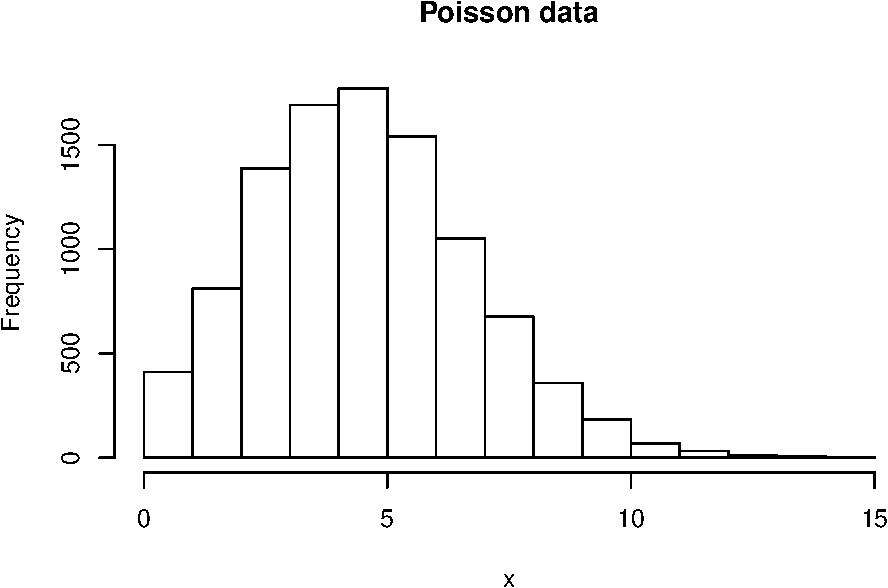
\includegraphics{call_center_data_files/figure-latex/poisson-1.pdf}

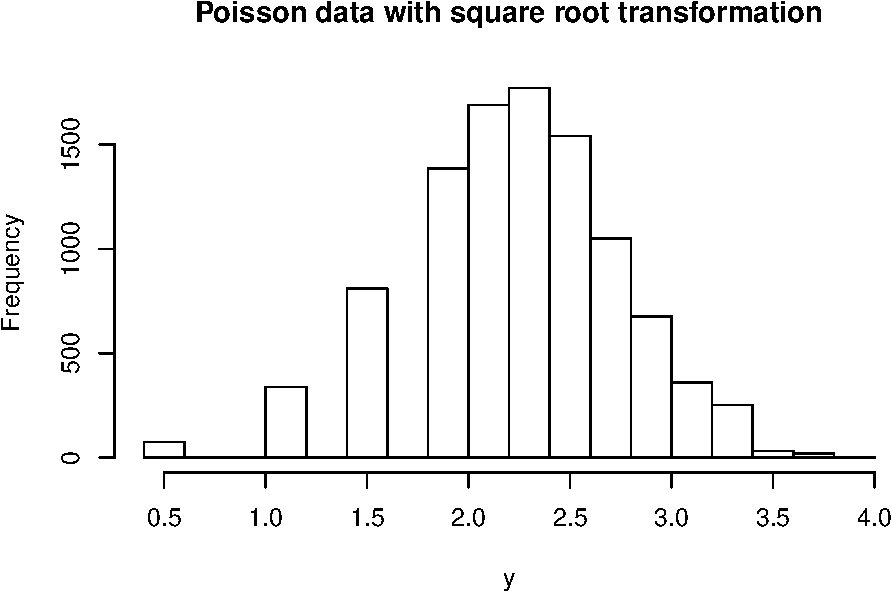
\includegraphics{call_center_data_files/figure-latex/normal-1.pdf}

Suppose we partition the covariance matrix of \(y\) as follows: \[
\Sigma = 
\begin{pmatrix}
\Sigma_{11} & \Sigma_{12} \\
\Sigma_{21} & \Sigma_{22} \\
\end{pmatrix}
\] In such a case,
\(y_2|y_1 \sim \mathcal{N}(\mu_2 + \Sigma_{21} \Sigma_{11}^{-1} (y_1 - \mu_1), \Sigma_{22} - \Sigma_{21} \Sigma_{11}^{-1} \Sigma_{12})\).
Hence the best mean squared predictor of \(y_2\) given \(y_1\) (i.e.~the
preidctor that minimizes mean squared error) is
\[\mathbb{E}[y_2|y_1] = \mu_2 + \Sigma_{21} \Sigma_{11}^{-1} (y_1 - \mu_1).\]
This is done using the follow code:

\begin{Shaded}
\begin{Highlighting}[]
\NormalTok{predict.mean <-}\StringTok{ }\ControlFlowTok{function}\NormalTok{(x1, mu, Sigma) \{}
\NormalTok{    p1 <-}\StringTok{ }\KeywordTok{length}\NormalTok{(x1)}
\NormalTok{    p <-}\StringTok{ }\KeywordTok{length}\NormalTok{(mu)}
\NormalTok{    p2 <-}\StringTok{ }\NormalTok{p }\OperatorTok{-}\StringTok{ }\NormalTok{p1}
\NormalTok{    mu1 <-}\StringTok{ }\NormalTok{mu[}\DecValTok{1}\OperatorTok{:}\NormalTok{p1]}
\NormalTok{    mu2 <-}\StringTok{ }\NormalTok{mu[(p1 }\OperatorTok{+}\StringTok{ }\DecValTok{1}\NormalTok{)}\OperatorTok{:}\NormalTok{p]}
\NormalTok{    Sigma11 <-}\StringTok{ }\NormalTok{Sigma[}\DecValTok{1}\OperatorTok{:}\NormalTok{p1, }\DecValTok{1}\OperatorTok{:}\NormalTok{p1]}
    \CommentTok{# Sigma12 <- Sigma[1:p1,(p1+1):p]}
\NormalTok{    Sigma21 <-}\StringTok{ }\NormalTok{Sigma[(p1 }\OperatorTok{+}\StringTok{ }\DecValTok{1}\NormalTok{)}\OperatorTok{:}\NormalTok{p, }\DecValTok{1}\OperatorTok{:}\NormalTok{p1]}
    \CommentTok{# Sigma22 <- Sigma[(p1+1):p,(p1+1):p]}
\NormalTok{    x2 <-}\StringTok{ }\NormalTok{mu2 }\OperatorTok{+}\StringTok{ }\NormalTok{Sigma21 }\OperatorTok\StringTok{ }\KeywordTok{solve}\NormalTok{(Sigma11, x1 }\OperatorTok{-}\StringTok{ }\NormalTok{mu1)}
    \KeywordTok{return}\NormalTok{(x2)}
\NormalTok{\}}
\end{Highlighting}
\end{Shaded}

Hence we must estimate \(\mu_2\) and \(\Sigma\) from the data. To this
end, we divide the dataset into a training datset and a test dataset.
Typically we do this in a random fashion, but since this is time-series
data, I take the first 70\% of the data to be the training dataset and
the remaining 30\% of the dataset to be the test dataset. Once we have
the estimates, we make predictions for the calls coming in for the
second half of the day using the calls that came in for the first half
of the day for the test data set and then compare with true values.

I divide the day up into 10 minute chunks and the first goal is to
reformat the data so that there is an easy way to view the number of
calls received at the call center on each day for each time period.

\begin{Shaded}
\begin{Highlighting}[]
\NormalTok{data =}\StringTok{ }\KeywordTok{filter}\NormalTok{(data, outcome }\OperatorTok{==}\StringTok{ "AGENT"}\NormalTok{)  ### keeping only agent outcome, rest are hangups or transforms(?!?)}
\NormalTok{data =}\StringTok{ }\KeywordTok{select}\NormalTok{(data, date, vru_entry)  ### only interested in date and vru entry. disccarding all other columns}
\NormalTok{data}\OperatorTok{$}\NormalTok{timedate =}\StringTok{ }\KeywordTok{paste}\NormalTok{(data}\OperatorTok{$}\NormalTok{date, data}\OperatorTok{$}\NormalTok{vru_entry)}
\NormalTok{data}\OperatorTok{$}\NormalTok{timedate =}\StringTok{ }\KeywordTok{strptime}\NormalTok{(data}\OperatorTok{$}\NormalTok{timedate, }\DataTypeTok{format =} \StringTok{"%y%m%d %H:%M:%S"}\NormalTok{)  ### converting to R date format}
\NormalTok{tt =}\StringTok{ }\KeywordTok{seq}\NormalTok{(}\DataTypeTok{from =} \KeywordTok{ISOdate}\NormalTok{(}\DecValTok{1999}\NormalTok{, }\DecValTok{1}\NormalTok{, }\DecValTok{1}\NormalTok{, }\DecValTok{0}\NormalTok{, }\DecValTok{0}\NormalTok{, }\DecValTok{0}\NormalTok{, }\DataTypeTok{tz =} \StringTok{"EST"}\NormalTok{), }\DataTypeTok{to =} \KeywordTok{ISOdate}\NormalTok{(}\DecValTok{1999}\NormalTok{, }
    \DecValTok{12}\NormalTok{, }\DecValTok{31}\NormalTok{, }\DecValTok{0}\NormalTok{, }\DecValTok{0}\NormalTok{, }\DecValTok{0}\NormalTok{, }\DataTypeTok{tz =} \StringTok{"EST"}\NormalTok{), }\DataTypeTok{by =} \StringTok{"10 min"}\NormalTok{)  ### creating 10 minute chunks}
\NormalTok{data}\OperatorTok{$}\NormalTok{timeperiods =}\StringTok{ }\KeywordTok{cut}\NormalTok{(data}\OperatorTok{$}\NormalTok{timedate, }\DataTypeTok{breaks =}\NormalTok{ tt)  ### dividing up calls accoridn to 10 minute chunks}

\NormalTok{data}\OperatorTok{$}\NormalTok{periods <-}\StringTok{ }\KeywordTok{sapply}\NormalTok{(}\KeywordTok{strsplit}\NormalTok{(}\KeywordTok{as.character}\NormalTok{(data}\OperatorTok{$}\NormalTok{timeperiods), }
    \StringTok{" "}\NormalTok{), }\StringTok{"["}\NormalTok{, }\DecValTok{2}\NormalTok{)  ### keeping only the time period. date discarded}

\NormalTok{data}\OperatorTok{$}\NormalTok{timeperiods <-}\StringTok{ }\KeywordTok{as.character}\NormalTok{(data}\OperatorTok{$}\NormalTok{timeperiods)}
\NormalTok{data}\OperatorTok{$}\NormalTok{count <-}\StringTok{ }\KeywordTok{as.numeric}\NormalTok{(}\KeywordTok{ave}\NormalTok{(data}\OperatorTok{$}\NormalTok{timeperiods, data}\OperatorTok{$}\NormalTok{timeperiods, }
    \DataTypeTok{FUN =}\NormalTok{ length))  ### creating a column with counts of how many calls were received in a certain time period}

\NormalTok{data2 =}\StringTok{ }\KeywordTok{select}\NormalTok{(data, date, periods, count)  ### keeping only relevant columns such as date, periods and counts.}

\NormalTok{data_wide <-}\StringTok{ }\KeywordTok{reshape}\NormalTok{(data2, }\DataTypeTok{timevar =} \StringTok{"periods"}\NormalTok{, }\DataTypeTok{idvar =} \KeywordTok{c}\NormalTok{(}\StringTok{"date"}\NormalTok{), }
    \DataTypeTok{direction =} \StringTok{"wide"}\NormalTok{)}

\NormalTok{data_wide[}\KeywordTok{is.na}\NormalTok{(data_wide)] =}\StringTok{ }\DecValTok{0}

\NormalTok{### reshaping long format to a wide format and setting all NA}
\NormalTok{### values to 0}

\NormalTok{#### reordering column by time}
\NormalTok{data_wide =}\StringTok{ }\NormalTok{data_wide[, }\KeywordTok{order}\NormalTok{(}\KeywordTok{names}\NormalTok{(data_wide))]}
\NormalTok{data_wide}\OperatorTok{$}\NormalTok{date2 =}\StringTok{ }\KeywordTok{strptime}\NormalTok{(data_wide}\OperatorTok{$}\NormalTok{date, }\DataTypeTok{format =} \StringTok{"%y%m%d"}\NormalTok{)}
\NormalTok{data_wide}\OperatorTok{$}\NormalTok{days =}\StringTok{ }\KeywordTok{weekdays}\NormalTok{(data_wide}\OperatorTok{$}\NormalTok{date2)  ### adding column for days of the week}
\NormalTok{data_wide}\OperatorTok{$}\NormalTok{holidays =}\StringTok{ }\DecValTok{1}\NormalTok{  ### adding a holidays column. 1 means not a holiday. 2 means a holiday. mostly for data visualization}

\CommentTok{# downloading list of holidays for 1999 for Israel}
\NormalTok{holidays =}\StringTok{ }\KeywordTok{readLines}\NormalTok{(}\StringTok{"http://world.std.com/~reinhold/jewishholidays.txt"}\NormalTok{)}
\NormalTok{holidays =}\StringTok{ }\NormalTok{holidays[}\KeywordTok{grepl}\NormalTok{(}\StringTok{"1999"}\NormalTok{, holidays)]}
\NormalTok{holidays =}\StringTok{ }\KeywordTok{unlist}\NormalTok{(}\KeywordTok{strsplit}\NormalTok{(holidays, }\StringTok{"}\CharTok{\textbackslash{}t}\StringTok{"}\NormalTok{))[}\KeywordTok{seq}\NormalTok{(}\DecValTok{1}\NormalTok{, }\DecValTok{28}\NormalTok{, }\DecValTok{2}\NormalTok{)]}
\NormalTok{holidays =}\StringTok{ }\KeywordTok{strptime}\NormalTok{(holidays, }\StringTok{"%a. %e %B %Y "}\NormalTok{)}


\ControlFlowTok{for}\NormalTok{ (i }\ControlFlowTok{in} \DecValTok{1}\OperatorTok{:}\KeywordTok{length}\NormalTok{(data_wide}\OperatorTok{$}\NormalTok{date2)) \{}
    \ControlFlowTok{for}\NormalTok{ (count }\ControlFlowTok{in} \DecValTok{1}\OperatorTok{:}\KeywordTok{length}\NormalTok{(holidays)) \{}
        \ControlFlowTok{if}\NormalTok{ (}\KeywordTok{sum}\NormalTok{(data_wide}\OperatorTok{$}\NormalTok{date2[i] }\OperatorTok{==}\StringTok{ }\NormalTok{holidays[count]) }\OperatorTok{>}\StringTok{ }\DecValTok{0}\NormalTok{) \{}
\NormalTok{            data_wide}\OperatorTok{$}\NormalTok{holidays[i] =}\StringTok{ }\DecValTok{2}
\NormalTok{        \}}
\NormalTok{    \}}
\NormalTok{\}}
\NormalTok{data_wide}\OperatorTok{$}\NormalTok{Colour =}\StringTok{ }\KeywordTok{ifelse}\NormalTok{(data_wide}\OperatorTok{$}\NormalTok{days }\OperatorTok{==}\StringTok{ "Friday"}\NormalTok{, }\DecValTok{1}\NormalTok{, }\KeywordTok{ifelse}\NormalTok{(data_wide}\OperatorTok{$}\NormalTok{days }\OperatorTok{==}\StringTok{ }
\StringTok{    "Monday"}\NormalTok{, }\DecValTok{2}\NormalTok{, }\KeywordTok{ifelse}\NormalTok{(data_wide}\OperatorTok{$}\NormalTok{days }\OperatorTok{==}\StringTok{ "Saturday"}\NormalTok{, }\DecValTok{3}\NormalTok{, }\KeywordTok{ifelse}\NormalTok{(data_wide}\OperatorTok{$}\NormalTok{days }\OperatorTok{==}\StringTok{ }
\StringTok{    "Sunday"}\NormalTok{, }\DecValTok{4}\NormalTok{, }\KeywordTok{ifelse}\NormalTok{(data_wide}\OperatorTok{$}\NormalTok{days }\OperatorTok{==}\StringTok{ "Thursday"}\NormalTok{, }\DecValTok{5}\NormalTok{, }\KeywordTok{ifelse}\NormalTok{(data_wide}\OperatorTok{$}\NormalTok{days }\OperatorTok{==}\StringTok{ }
\StringTok{    "Tuesday"}\NormalTok{, }\DecValTok{6}\NormalTok{, }\DecValTok{7}\NormalTok{))))))  ### adding a colour column based on day of week}

\NormalTok{#### deleting all times before 7AM when the center opens and}
\NormalTok{#### date column and convert data to matrix format}
\NormalTok{X =}\StringTok{ }\KeywordTok{as.matrix}\NormalTok{(data_wide[, }\OperatorTok{-}\KeywordTok{c}\NormalTok{(}\DecValTok{1}\OperatorTok{:}\DecValTok{29}\NormalTok{, }\DecValTok{132}\OperatorTok{:}\DecValTok{137}\NormalTok{)])}
\NormalTok{Xsvd =}\StringTok{ }\KeywordTok{svd}\NormalTok{(X)}
\NormalTok{data_wide}\OperatorTok{$}\NormalTok{date2 <-}\StringTok{ }\KeywordTok{as.POSIXct}\NormalTok{(data_wide}\OperatorTok{$}\NormalTok{date2)}
\NormalTok{data_fri =}\StringTok{ }\KeywordTok{filter}\NormalTok{(data_wide, days }\OperatorTok{==}\StringTok{ "Friday"}\NormalTok{)}
\KeywordTok{dim}\NormalTok{(data_fri)}
\end{Highlighting}
\end{Shaded}

\begin{verbatim}
## [1]  52 137
\end{verbatim}

\begin{Shaded}
\begin{Highlighting}[]
\NormalTok{data_sat =}\StringTok{ }\KeywordTok{filter}\NormalTok{(data_wide, days }\OperatorTok{==}\StringTok{ "Saturday"}\NormalTok{)}
\NormalTok{data_rest =}\StringTok{ }\KeywordTok{filter}\NormalTok{(data_wide, days }\OperatorTok{!=}\StringTok{ "Saturday"} \OperatorTok{&}\StringTok{ }\NormalTok{days }\OperatorTok{!=}\StringTok{ "Friday"}\NormalTok{)}
\NormalTok{X =}\StringTok{ }\KeywordTok{as.matrix}\NormalTok{(data_wide[, }\OperatorTok{-}\KeywordTok{c}\NormalTok{(}\DecValTok{1}\OperatorTok{:}\DecValTok{29}\NormalTok{, }\DecValTok{132}\OperatorTok{:}\DecValTok{137}\NormalTok{)])}
\NormalTok{X_fri =}\StringTok{ }\KeywordTok{as.matrix}\NormalTok{(data_fri[, }\OperatorTok{-}\KeywordTok{c}\NormalTok{(}\DecValTok{1}\OperatorTok{:}\DecValTok{29}\NormalTok{, }\DecValTok{132}\OperatorTok{:}\DecValTok{137}\NormalTok{)])}
\NormalTok{X_sat =}\StringTok{ }\KeywordTok{as.matrix}\NormalTok{(data_sat[, }\OperatorTok{-}\KeywordTok{c}\NormalTok{(}\DecValTok{1}\OperatorTok{:}\DecValTok{29}\NormalTok{, }\DecValTok{132}\OperatorTok{:}\DecValTok{137}\NormalTok{)])}
\NormalTok{X_rest =}\StringTok{ }\KeywordTok{as.matrix}\NormalTok{(data_rest[, }\OperatorTok{-}\KeywordTok{c}\NormalTok{(}\DecValTok{1}\OperatorTok{:}\DecValTok{29}\NormalTok{, }\DecValTok{132}\OperatorTok{:}\DecValTok{137}\NormalTok{)])}
\NormalTok{#### for poisson data apply transformation sqrt(x+1/4) to data}
\NormalTok{#### to make more normal}
\NormalTok{Y =}\StringTok{ }\KeywordTok{sqrt}\NormalTok{(X }\OperatorTok{+}\StringTok{ }\DecValTok{1}\OperatorTok{/}\DecValTok{4}\NormalTok{)}
\NormalTok{Y_fri =}\StringTok{ }\KeywordTok{sqrt}\NormalTok{(X_fri }\OperatorTok{+}\StringTok{ }\DecValTok{1}\OperatorTok{/}\DecValTok{4}\NormalTok{)}
\NormalTok{Y_sat =}\StringTok{ }\KeywordTok{sqrt}\NormalTok{(X_sat }\OperatorTok{+}\StringTok{ }\DecValTok{1}\OperatorTok{/}\DecValTok{4}\NormalTok{)}
\NormalTok{Y_rest =}\StringTok{ }\KeywordTok{sqrt}\NormalTok{(X_rest }\OperatorTok{+}\StringTok{ }\DecValTok{1}\OperatorTok{/}\DecValTok{4}\NormalTok{)}
\end{Highlighting}
\end{Shaded}

\subsubsection{Scree Plots}\label{scree-plots}

The scree plot indicates that about 25\% is explained by the 1st
eigenvector, about 5\% by the 2nd one and so on.

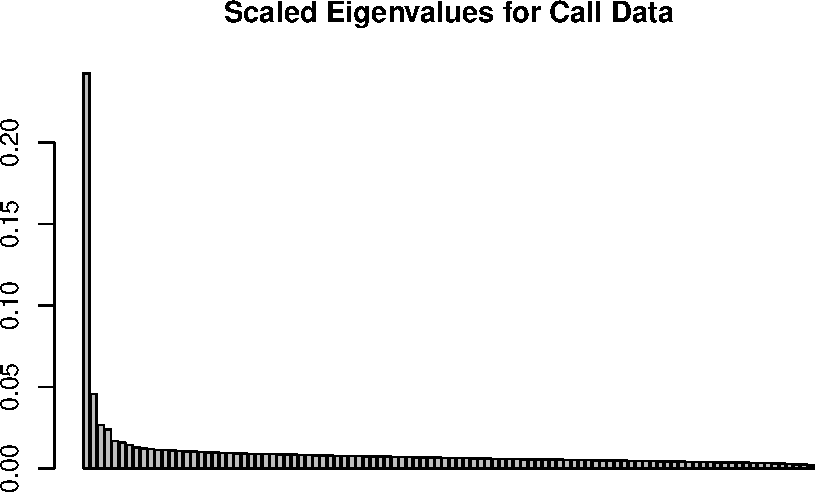
\includegraphics{call_center_data_files/figure-latex/scree-1.pdf}

\subsubsection{Bi-Plots}\label{bi-plots}

The bi-plot indicates that the weekends (Fridays and Saturdays in
Israel) are separate from the rest of the data. This indicates that for
the prediction phase, it might be best to work on all of these
separately. The triangles indicate +/-1 day from Holidays. Almost all
the outlier seem to be either the weekends or Holidays.

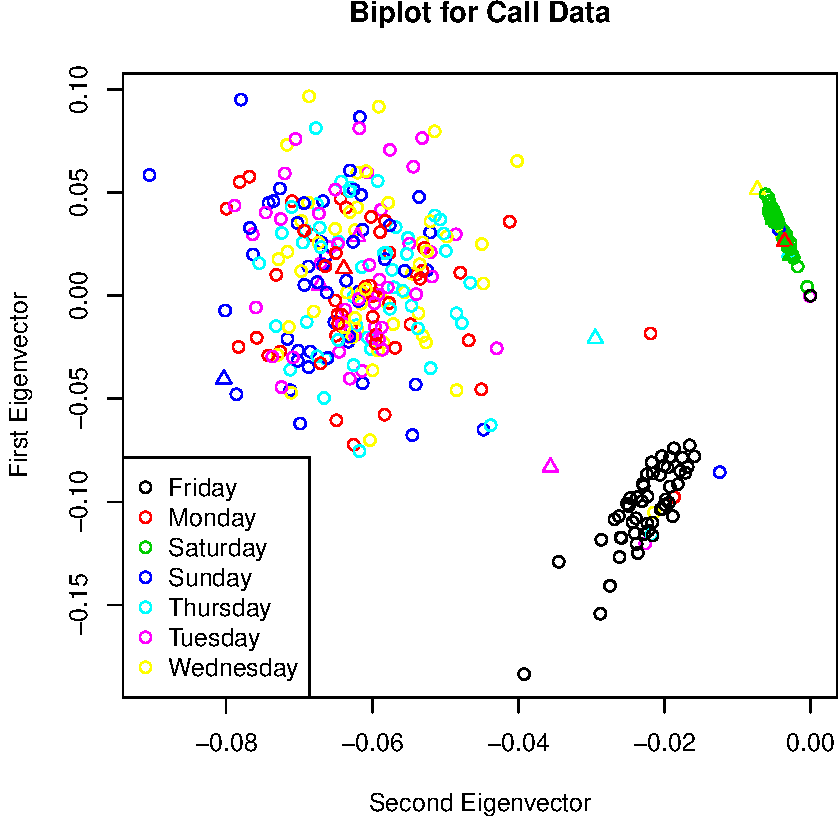
\includegraphics{call_center_data_files/figure-latex/biplot-1.pdf}

\subsubsection{Model Evaluation}\label{model-evaluation}

To evaulate the models we use Absolute Error(AE) where

\[
AE_t = \frac{1}{T}\sum_{i = T+1}^{364} |\hat{y}_{it} - y_{it}|
\]

and \(T\) is the size of the training dataset.

\subsubsection{Full dataset}\label{full-dataset}

Initially we do the evaluations on the full dataset (including
weekends). We estimate \(\mu_2\) by using the sample mean and estimate
\(\Sigma\) using the sample covariance method and CSCS. For CSCS, we
need to pick a penalty parameter, which we do using cross-validation of
the likelihood.

\begin{Shaded}
\begin{Highlighting}[]
\NormalTok{CSCS2 <-}\StringTok{ }\ControlFlowTok{function}\NormalTok{(Y, lambda, }\DataTypeTok{L =} \OtherTok{NULL}\NormalTok{, }\DataTypeTok{maxitr =} \DecValTok{100}\NormalTok{, }\DataTypeTok{tol =} \FloatTok{1e-04}\NormalTok{, }
    \DataTypeTok{warmstart =} \OtherTok{FALSE}\NormalTok{) \{}
    
\NormalTok{    #### inputs Y: n by p matrix of data lambda: l1-penalty}
\NormalTok{    #### parameter maxitr: maximum number of iterations allowed}
\NormalTok{    #### (diagonal/off-diagonal optimization) tol: if maximum}
\NormalTok{    #### difference of iterates is less than tol, consider converged}
\NormalTok{    #### warmstart: warmstarting actually made the runs slower}
\NormalTok{    #### (overhead may be too expensive)}
    
\NormalTok{    #### outputs L: lower triangular matrix of cholesky factor}
\NormalTok{    #### computed with CSCS algorithm itr_log: (p-1)-vector of}
\NormalTok{    #### number of iterations eps_log: (p-1)-vector of number}
\NormalTok{    #### maximum difference for considering convergence}
    
    
\NormalTok{    n =}\StringTok{ }\KeywordTok{nrow}\NormalTok{(Y)}
\NormalTok{    p =}\StringTok{ }\KeywordTok{ncol}\NormalTok{(Y)}
    
    \ControlFlowTok{if}\NormalTok{ (}\KeywordTok{is.null}\NormalTok{(L)) }
\NormalTok{        L =}\StringTok{ }\KeywordTok{diag}\NormalTok{(p)}
    
\NormalTok{    S =}\StringTok{ }\NormalTok{(}\KeywordTok{t}\NormalTok{(Y) }\OperatorTok\StringTok{ }\NormalTok{Y)}\OperatorTok{/}\NormalTok{n}
    
\NormalTok{    itr_log =}\StringTok{ }\NormalTok{eps_log =}\StringTok{ }\OtherTok{NULL}
    
\NormalTok{    L[}\DecValTok{1}\NormalTok{, }\DecValTok{1}\NormalTok{] =}\StringTok{ }\DecValTok{1}\OperatorTok{/}\KeywordTok{sqrt}\NormalTok{(S[}\DecValTok{1}\NormalTok{, }\DecValTok{1}\NormalTok{])}
    \ControlFlowTok{for}\NormalTok{ (k }\ControlFlowTok{in} \DecValTok{2}\OperatorTok{:}\NormalTok{p) \{}
\NormalTok{        ## Loop in Algorithm 2}
        
\NormalTok{        ## nu_k vector (equation 2.5)}
\NormalTok{        nuk_old =}\StringTok{ }\NormalTok{nuk_new =}\StringTok{ }\KeywordTok{c}\NormalTok{(}\KeywordTok{rep}\NormalTok{(}\DecValTok{0}\NormalTok{, k }\OperatorTok{-}\StringTok{ }\DecValTok{1}\NormalTok{), }\DecValTok{1}\NormalTok{)}
\NormalTok{        r =}\StringTok{ }\DecValTok{0}
        
        \ControlFlowTok{repeat}\NormalTok{ \{}
\NormalTok{            ## Loop in Algorithm 1}
            
\NormalTok{            r =}\StringTok{ }\NormalTok{r }\OperatorTok{+}\StringTok{ }\DecValTok{1}
            
\NormalTok{            km1_ =}\StringTok{ }\DecValTok{1}\OperatorTok{:}\NormalTok{(k }\OperatorTok{-}\StringTok{ }\DecValTok{1}\NormalTok{)  ## 1, ..., k-1 is off-diagonal elements indices}
            
\NormalTok{            ## Update off-diagonal terms}
\NormalTok{            hk =}\StringTok{ }\KeywordTok{lassoshooting}\NormalTok{(}\DataTypeTok{XtX =}\NormalTok{ S[km1_, km1_, }\DataTypeTok{drop =} \OtherTok{FALSE}\NormalTok{], }
                \DataTypeTok{Xty =} \OperatorTok{-}\NormalTok{nuk_old[k] }\OperatorTok{*}\StringTok{ }\NormalTok{S[km1_, k], }\DataTypeTok{lambda =} \FloatTok{0.5} \OperatorTok{*}\StringTok{ }
\StringTok{                  }\NormalTok{lambda)}
\NormalTok{            nuk_new[km1_] =}\StringTok{ }\NormalTok{hk}\OperatorTok{$}\NormalTok{coefficients}
            
\NormalTok{            ## Update diagonal term}
\NormalTok{            sumterm =}\StringTok{ }\KeywordTok{sum}\NormalTok{(nuk_new[km1_] }\OperatorTok{*}\StringTok{ }\NormalTok{S[k, km1_])}
\NormalTok{            nuk_new[k] =}\StringTok{ }\NormalTok{(}\OperatorTok{-}\NormalTok{sumterm }\OperatorTok{+}\StringTok{ }\KeywordTok{sqrt}\NormalTok{(sumterm}\OperatorTok{^}\DecValTok{2} \OperatorTok{+}\StringTok{ }\DecValTok{4} \OperatorTok{*}\StringTok{ }\NormalTok{S[k, }
\NormalTok{                k]))}\OperatorTok{/}\NormalTok{(}\DecValTok{2} \OperatorTok{*}\StringTok{ }\NormalTok{S[k, k])}
            
\NormalTok{            ## Check convergence}
\NormalTok{            maxdiff =}\StringTok{ }\KeywordTok{max}\NormalTok{(}\KeywordTok{abs}\NormalTok{(nuk_new }\OperatorTok{-}\StringTok{ }\NormalTok{nuk_old))}
            \ControlFlowTok{if}\NormalTok{ (maxdiff }\OperatorTok{<}\StringTok{ }\NormalTok{tol }\OperatorTok{||}\StringTok{ }\NormalTok{r }\OperatorTok{>=}\StringTok{ }\NormalTok{maxitr) \{}
\NormalTok{                L[k, }\DecValTok{1}\OperatorTok{:}\NormalTok{k] =}\StringTok{ }\NormalTok{nuk_new}
\NormalTok{                eps_log =}\StringTok{ }\KeywordTok{c}\NormalTok{(eps_log, maxdiff)}
\NormalTok{                itr_log =}\StringTok{ }\KeywordTok{c}\NormalTok{(itr_log, r)}
                \ControlFlowTok{break}
\NormalTok{            \} }\ControlFlowTok{else}\NormalTok{ \{}
\NormalTok{                nuk_old =}\StringTok{ }\NormalTok{nuk_new}
\NormalTok{            \}}
\NormalTok{        \}}
\NormalTok{    \}}
    
    \KeywordTok{list}\NormalTok{(}\DataTypeTok{L =}\NormalTok{ L, }\DataTypeTok{itr =}\NormalTok{ itr_log, }\DataTypeTok{eps =}\NormalTok{ eps_log)}
    
\NormalTok{\}}
\end{Highlighting}
\end{Shaded}

\begin{Shaded}
\begin{Highlighting}[]
\NormalTok{cv =}\StringTok{ }\ControlFlowTok{function}\NormalTok{(lambda, K, train) \{}
\NormalTok{    cvec =}\StringTok{ }\KeywordTok{rep}\NormalTok{(}\DecValTok{0}\NormalTok{, K)}
    \KeywordTok{set.seed}\NormalTok{(}\DecValTok{12345}\NormalTok{)}
\NormalTok{    index =}\StringTok{ }\KeywordTok{sample}\NormalTok{(}\DecValTok{1}\OperatorTok{:}\KeywordTok{dim}\NormalTok{(train)[}\DecValTok{1}\NormalTok{], }\DataTypeTok{replace =} \OtherTok{FALSE}\NormalTok{)}
\NormalTok{    foldsize =}\StringTok{ }\KeywordTok{ceiling}\NormalTok{(}\KeywordTok{dim}\NormalTok{(train)[}\DecValTok{1}\NormalTok{]}\OperatorTok{/}\NormalTok{K)}
\NormalTok{    inTrain <-}\StringTok{ }\KeywordTok{list}\NormalTok{()}
    \ControlFlowTok{for}\NormalTok{ (i }\ControlFlowTok{in} \DecValTok{1}\OperatorTok{:}\NormalTok{(K }\OperatorTok{-}\StringTok{ }\DecValTok{1}\NormalTok{)) \{}
\NormalTok{        inTrain[[i]] <-}\StringTok{ }\NormalTok{index[((i }\OperatorTok{-}\StringTok{ }\DecValTok{1}\NormalTok{) }\OperatorTok{*}\StringTok{ }\NormalTok{foldsize }\OperatorTok{+}\StringTok{ }\DecValTok{1}\NormalTok{)}\OperatorTok{:}\NormalTok{((i }\OperatorTok{-}\StringTok{ }
\StringTok{            }\DecValTok{1}\NormalTok{) }\OperatorTok{*}\StringTok{ }\NormalTok{foldsize }\OperatorTok{+}\StringTok{ }\NormalTok{foldsize)]}
\NormalTok{    \}}
\NormalTok{    inTrain[[K]] <-}\StringTok{ }\NormalTok{index[((K }\OperatorTok{-}\StringTok{ }\DecValTok{1}\NormalTok{) }\OperatorTok{*}\StringTok{ }\NormalTok{foldsize }\OperatorTok{+}\StringTok{ }\DecValTok{1}\NormalTok{)}\OperatorTok{:}\KeywordTok{length}\NormalTok{(index)]}
    \ControlFlowTok{for}\NormalTok{ (k }\ControlFlowTok{in} \DecValTok{1}\OperatorTok{:}\NormalTok{K) \{}
\NormalTok{        Ytrain =}\StringTok{ }\NormalTok{train[}\OperatorTok{-}\KeywordTok{c}\NormalTok{(inTrain[[k]]), ]}
\NormalTok{        Ytest =}\StringTok{ }\NormalTok{train[}\KeywordTok{c}\NormalTok{(inTrain[[k]]), ]}
\NormalTok{        E =}\StringTok{ }\NormalTok{Ytrain}
\NormalTok{        out =}\StringTok{ }\KeywordTok{CSCS2}\NormalTok{(}\KeywordTok{as.matrix}\NormalTok{(E), lambda)}\OperatorTok{$}\NormalTok{L}
\NormalTok{        Sigma_v =}\StringTok{ }\KeywordTok{t}\NormalTok{(out) }\OperatorTok\StringTok{ }\NormalTok{out}
\NormalTok{        s_v =}\StringTok{ }\KeywordTok{dim}\NormalTok{(Ytest)[}\DecValTok{1}\NormalTok{]}
\NormalTok{        sumterm =}\StringTok{ }\KeywordTok{sum}\NormalTok{(}\KeywordTok{diag}\NormalTok{(Ytest }\OperatorTok\StringTok{ }\NormalTok{(Sigma_v) }\OperatorTok\StringTok{ }\KeywordTok{t}\NormalTok{(Ytest)))}
\NormalTok{        cvec[k] =}\StringTok{ }\NormalTok{s_v }\OperatorTok{*}\StringTok{ }\KeywordTok{log}\NormalTok{(}\KeywordTok{det}\NormalTok{(}\KeywordTok{solve}\NormalTok{(Sigma_v))) }\OperatorTok{+}\StringTok{ }\NormalTok{sumterm}
\NormalTok{    \}}
\NormalTok{    cv =}\StringTok{ }\NormalTok{(}\DecValTok{1}\OperatorTok{/}\NormalTok{K) }\OperatorTok{*}\StringTok{ }\KeywordTok{sum}\NormalTok{(cvec)}
    \KeywordTok{return}\NormalTok{(cv)}
\NormalTok{\}}
\end{Highlighting}
\end{Shaded}

\begin{Shaded}
\begin{Highlighting}[]
\NormalTok{training =}\StringTok{ }\DecValTok{1}\OperatorTok{:}\DecValTok{252}
\NormalTok{train =}\StringTok{ }\KeywordTok{scale}\NormalTok{(Y[training, ], }\DataTypeTok{center =} \OtherTok{TRUE}\NormalTok{, }\DataTypeTok{scale =} \OtherTok{FALSE}\NormalTok{)}
\NormalTok{test =}\StringTok{ }\NormalTok{Y[}\OperatorTok{-}\NormalTok{training, ]}
\NormalTok{mu =}\StringTok{ }\KeywordTok{colMeans}\NormalTok{(train)}
\NormalTok{S =}\StringTok{ }\NormalTok{(}\KeywordTok{t}\NormalTok{(train) }\OperatorTok\StringTok{ }\NormalTok{train)}\OperatorTok{/}\NormalTok{(}\KeywordTok{dim}\NormalTok{(train)[}\DecValTok{1}\NormalTok{])}
\NormalTok{SError <-}\StringTok{ }\KeywordTok{matrix}\NormalTok{(}\DecValTok{0}\NormalTok{, }\DataTypeTok{nrow =} \KeywordTok{nrow}\NormalTok{(test), }\DataTypeTok{ncol =} \DecValTok{51}\NormalTok{)}
\ControlFlowTok{for}\NormalTok{ (k }\ControlFlowTok{in} \DecValTok{1}\OperatorTok{:}\KeywordTok{nrow}\NormalTok{(test)) \{}
\NormalTok{    S.mu2 <-}\StringTok{ }\KeywordTok{predict.mean}\NormalTok{(test[k, }\DecValTok{1}\OperatorTok{:}\DecValTok{51}\NormalTok{], }\DataTypeTok{mu =}\NormalTok{ mu, }\DataTypeTok{Sigma =}\NormalTok{ S)}
\NormalTok{    SError[k, ] <-}\StringTok{ }\NormalTok{(S.mu2 }\OperatorTok{-}\StringTok{ }\KeywordTok{as.numeric}\NormalTok{(test[k, }\DecValTok{52}\OperatorTok{:}\DecValTok{102}\NormalTok{]))}
\NormalTok{\}}
\NormalTok{E.S <-}\StringTok{ }\KeywordTok{colMeans}\NormalTok{(}\KeywordTok{abs}\NormalTok{(SError))}
\NormalTok{Time =}\StringTok{ }\DecValTok{52}\OperatorTok{:}\DecValTok{102}
\NormalTok{AE =}\StringTok{ }\NormalTok{E.S}
\NormalTok{Method =}\StringTok{ }\KeywordTok{rep}\NormalTok{(}\StringTok{"S"}\NormalTok{, }\KeywordTok{length}\NormalTok{(AE))}
\NormalTok{Sdata =}\StringTok{ }\KeywordTok{data.frame}\NormalTok{(Method, AE, Time)}

\NormalTok{lambdal =}\StringTok{ }\FloatTok{0.01}
\NormalTok{lambda =}\StringTok{ }\KeywordTok{seq}\NormalTok{(}\FloatTok{0.1}\NormalTok{, }\FloatTok{0.2}\NormalTok{, }\DataTypeTok{by =}\NormalTok{ lambdal)}
\NormalTok{out =}\StringTok{ }\KeywordTok{rep}\NormalTok{(}\DecValTok{0}\NormalTok{, }\KeywordTok{length}\NormalTok{(lambda))}
\ControlFlowTok{for}\NormalTok{ (k }\ControlFlowTok{in} \DecValTok{1}\OperatorTok{:}\KeywordTok{length}\NormalTok{(lambda)) \{}
\NormalTok{    out[k] =}\StringTok{ }\KeywordTok{cv}\NormalTok{(lambda[k], }\DecValTok{5}\NormalTok{, train)}
\NormalTok{\}}
\end{Highlighting}
\end{Shaded}

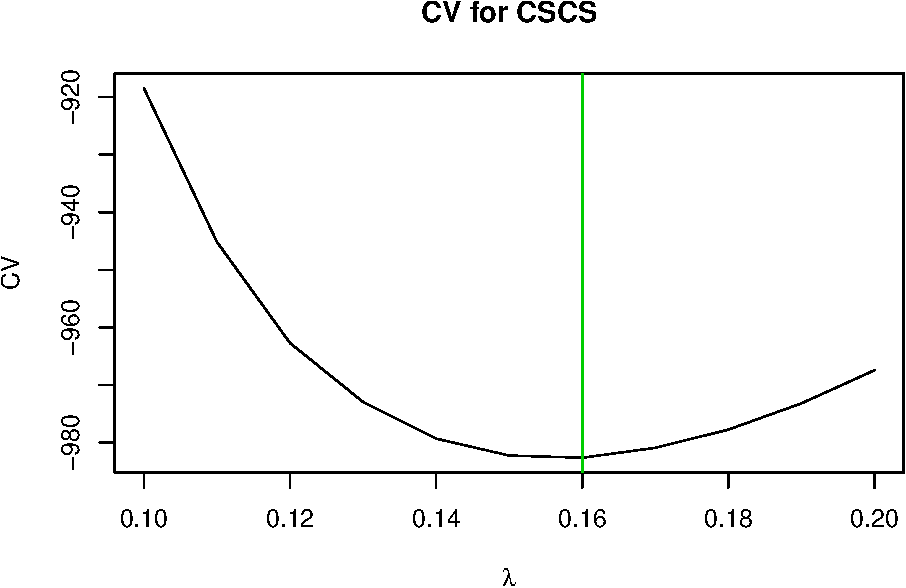
\includegraphics{call_center_data_files/figure-latex/plot-1.pdf}

\begin{Shaded}
\begin{Highlighting}[]
\NormalTok{lambdastar =}\StringTok{ }\NormalTok{lambda[}\KeywordTok{which.min}\NormalTok{(out)]}
\NormalTok{E =}\StringTok{ }\NormalTok{train}
\NormalTok{out =}\StringTok{ }\KeywordTok{CSCS2}\NormalTok{(}\KeywordTok{as.matrix}\NormalTok{(E), lambdastar)}\OperatorTok{$}\NormalTok{L}
\NormalTok{CSCS =}\StringTok{ }\KeywordTok{solve}\NormalTok{(}\KeywordTok{t}\NormalTok{(out) }\OperatorTok\StringTok{ }\NormalTok{out)}
\NormalTok{CSCSError <-}\StringTok{ }\KeywordTok{matrix}\NormalTok{(}\DecValTok{0}\NormalTok{, }\DataTypeTok{nrow =} \KeywordTok{nrow}\NormalTok{(test), }\DataTypeTok{ncol =} \DecValTok{51}\NormalTok{)}
\ControlFlowTok{for}\NormalTok{ (k }\ControlFlowTok{in} \DecValTok{1}\OperatorTok{:}\KeywordTok{nrow}\NormalTok{(test)) \{}
\NormalTok{    CSCS.mu2 <-}\StringTok{ }\KeywordTok{predict.mean}\NormalTok{(test[k, }\DecValTok{1}\OperatorTok{:}\DecValTok{51}\NormalTok{], }\DataTypeTok{mu =}\NormalTok{ mu, }\DataTypeTok{Sigma =}\NormalTok{ CSCS)}
\NormalTok{    CSCSError[k, ] <-}\StringTok{ }\NormalTok{(CSCS.mu2 }\OperatorTok{-}\StringTok{ }\KeywordTok{as.numeric}\NormalTok{(test[k, }\DecValTok{52}\OperatorTok{:}\DecValTok{102}\NormalTok{]))}
\NormalTok{\}}
\NormalTok{E.CSCS <-}\StringTok{ }\KeywordTok{colMeans}\NormalTok{(}\KeywordTok{abs}\NormalTok{(CSCSError))}
\NormalTok{Time =}\StringTok{ }\DecValTok{52}\OperatorTok{:}\DecValTok{102}
\NormalTok{AE =}\StringTok{ }\NormalTok{E.CSCS}
\NormalTok{Method =}\StringTok{ }\KeywordTok{rep}\NormalTok{(}\StringTok{"CSCS"}\NormalTok{, }\KeywordTok{length}\NormalTok{(AE))}
\NormalTok{CSCSdata =}\StringTok{ }\KeywordTok{data.frame}\NormalTok{(Method, AE, Time)}
\end{Highlighting}
\end{Shaded}

The following plot shows the comparison of using the sample covariance
matrix and CSCS on the full dataset. It's quite clear that CSCS does
better than the sample covariance matrix in most cases.

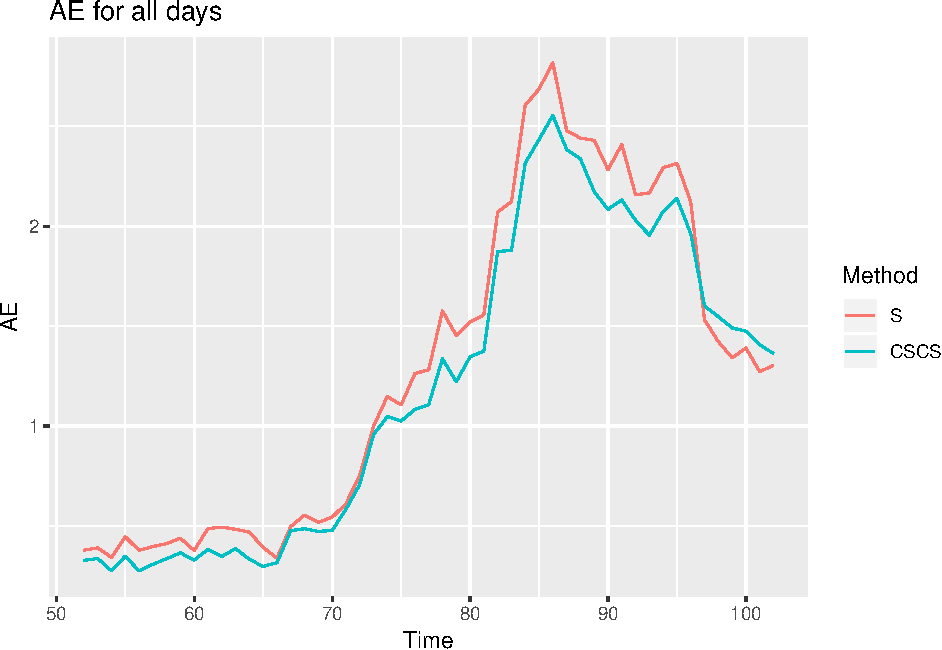
\includegraphics{call_center_data_files/figure-latex/comp1-1.pdf}

\subsubsection{Weekdays}\label{weekdays}

This is the comparison for just the weekdays. Here, there isn't a clear
winner. This is probably our dataset is more homogenous. CSCS is a more
robust covariance estimator than the sample covaraince matrix. As we
focussed on dataset with fewer outliers, the sample covariance matrix
performed better comparitively.

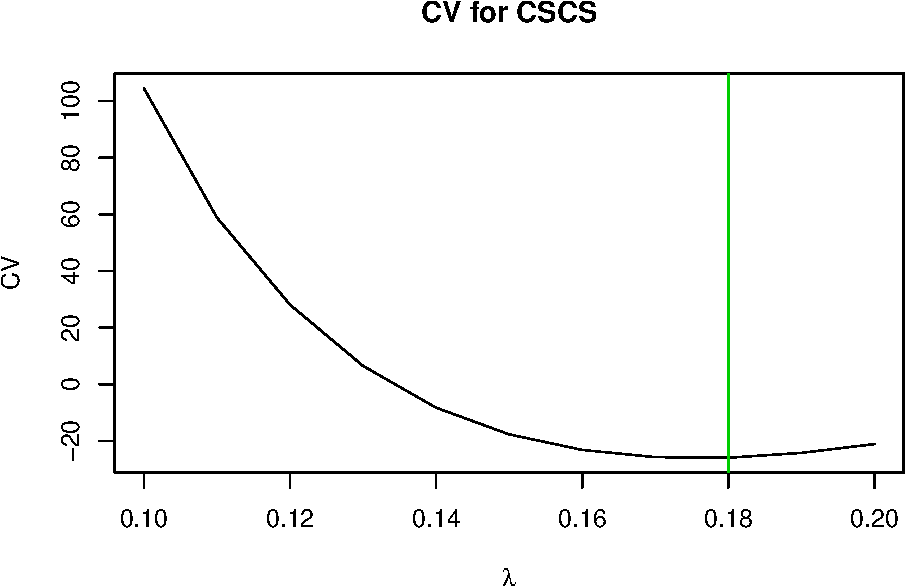
\includegraphics{call_center_data_files/figure-latex/unnamed-chunk-1-1.pdf}

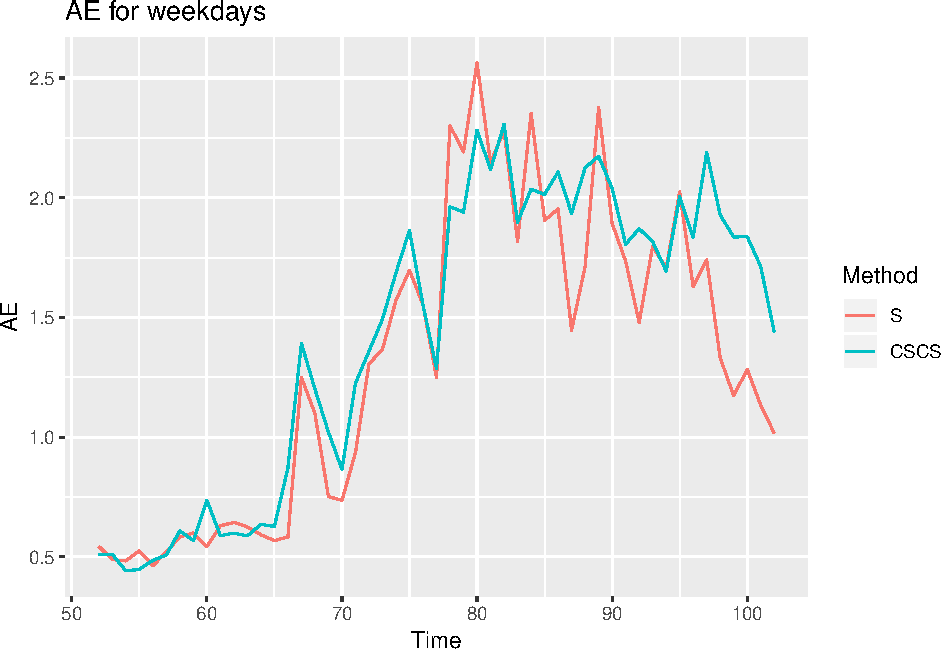
\includegraphics{call_center_data_files/figure-latex/weekdaycont-1.pdf}

\subsubsection{Connections to graphical
models}\label{connections-to-graphical-models}

Finally, below is a graph showing how the time periods are related.
Here, Node \(i\) corresponds to Time Period \(i\).

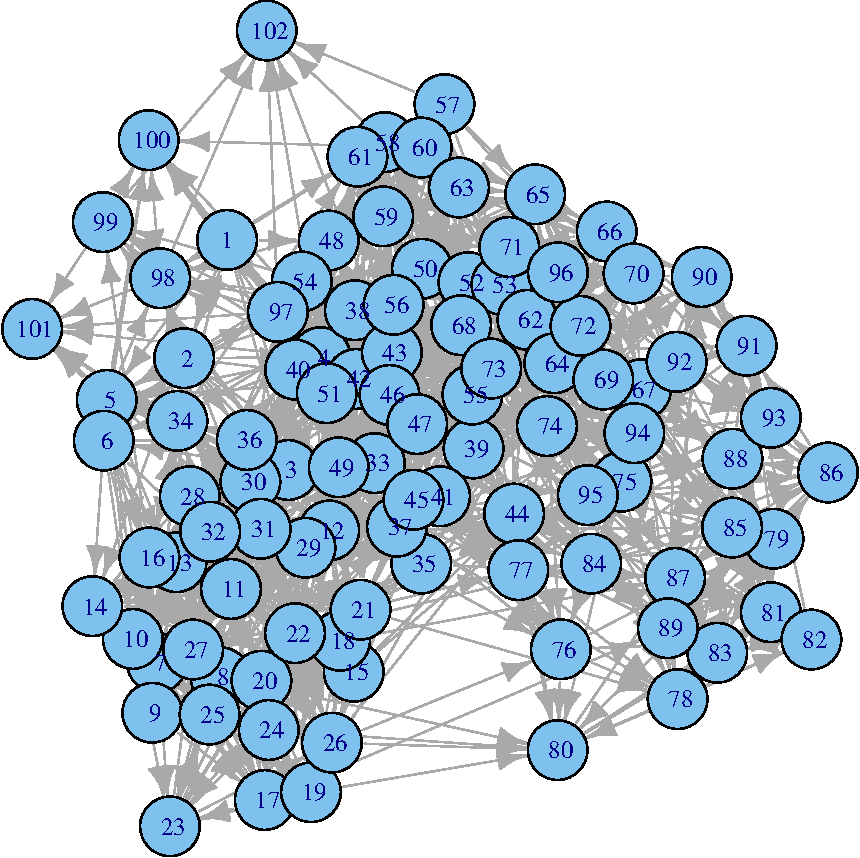
\includegraphics{call_center_data_files/figure-latex/graph-1.pdf}


\end{document}
